\chapter{Đọc thêm: Rủi ro và Lợi suất (Dahlquist \& Knight)}
\label{ch:M3L1-reading1}

% Nguồn: Dahlquist, Julie, and Rainford Knight. "Principles of Finance." OpenStax, 2022.
% Phần cần đọc: Sections 15.1 (Risk and Return to an Individual Asset) & 15.2 (Risk and Return to Multiple Assets)
% Nội dung bắt buộc đọc: được kiểm tra trong mọi bài đánh giá (kể cả Quiz).

\section{Thông tin nguồn}

\begin{itemize}
  \item \textbf{Nguồn:} Dahlquist, Julie, and Rainford Knight. \emph{Principles of Finance}. OpenStax Press, 2022. (truy cập mở tại \url{https://openstax.org/details/books/principles-finance})
  \item \textbf{Phần cần đọc:} Section 15.1: Risk and Return to an Individual Asset; Section 15.2: Risk and Return to Multiple Assets
\end{itemize}

\section{15.1 Rủi ro và Lợi suất của Một Tài sản Riêng lẻ}

\subsection*{Mục tiêu học tập}
Sau khi hoàn thành mục này, bạn sẽ có thể:
\begin{itemize}
  \item Tính lợi suất thực hiện (realized return) từ một khoản đầu tư riêng lẻ.
  \item Tính lợi suất trung bình và độ biến động của lợi suất từ dữ liệu lịch sử.
  \item Mô tả rủi ro đặc thù doanh nghiệp (firm-specific risk).
\end{itemize}

\subsection*{Đo lường Lợi suất Lịch sử}

Rủi ro và lợi suất thường được gọi là hai chữ R (the two Rs) của tài chính. Nhà đầu tư quan tâm đến cả rủi ro lẫn lợi suất vì hiểu một cái mà không hiểu cái kia thì thực sự vô nghĩa. Về mặt đầu tư, khái niệm lợi suất khá đơn giản: lợi suất là lợi ích, hay lợi nhuận, mà nhà đầu tư kỳ vọng từ một khoản chi tiêu. Đó là phần thưởng cho việc đầu tư — lý do khiến một khoản đầu tư được thực hiện ngay từ đầu. Tuy nhiên, không có khoản đầu tư nào là chắc chắn. Lợi suất thực tế có thể không như nhà đầu tư kỳ vọng. Sự không chắc chắn về lợi suất này được gọi là rủi ro.

Chúng ta bắt đầu bằng cách xem xét cách đo lường cả rủi ro lẫn lợi suất khi xét một tài sản riêng lẻ, chẳng hạn một cổ phiếu. Nếu ông bà bạn mua 100 cổ phiếu Apple, Inc. cho bạn khi bạn mới sinh ra, bạn sẽ muốn biết khoản đầu tư đó đã sinh lời tốt đến đâu. Bạn thậm chí có thể muốn so sánh khoản đầu tư đó với một khoản đầu tư vào một cổ phiếu khác, chẳng hạn Disney, xem cái nào tốt hơn. Bạn quan tâm đến việc đo lường lợi suất lịch sử.

\subsection*{Lợi suất Thực hiện của Khoản đầu tư Riêng lẻ}

Lợi suất thực hiện (realized return) của một khoản đầu tư là tổng lợi suất xảy ra trong một khoảng thời gian cụ thể. Giả sử bạn mua một cổ phiếu Target (TGT) vào đầu tháng 1/2020 với giá \$128.74. Đến cuối năm, bạn bán cổ phiếu với giá \$176.53, cao hơn \$47.79 so với giá mua. Mức tăng giá trị này được gọi là lãi vốn (capital gain). Là chủ sở hữu cổ phiếu, bạn cũng nhận được \$2.68 cổ tức trong năm 2020. Tổng lợi suất bằng đô la từ khoản đầu tư của bạn được tính như sau:

$$
\text{Tổng lợi suất} = \$47.79 + \$2.68 = \$50.47
$$

Lợi suất đầu tư thường được biểu diễn theo phần trăm thay vì đô la. Điều này cho phép bạn trả lời câu hỏi "Tôi nhận được bao nhiêu cho mỗi đô la đầu tư?" để có thể so sánh các khoản đầu tư có quy mô khác nhau. Tổng lợi suất phần trăm từ khoản đầu tư của bạn là:

$$
\text{Tổng lợi suất \%} = \frac{\$50.47}{\$128.74} = 39.20\%
$$

Tỷ suất cổ tức (dividend yield) được tính bằng cách chia cổ tức nhận được cho giá cổ phiếu ban đầu. Phép tính này cho thấy với mỗi đô la đầu tư vào TGT năm 2020, bạn nhận được \$0.0208 tiền cổ tức. Tỷ suất lãi vốn (capital gain yield) là mức thay đổi giá cổ phiếu chia cho giá cổ phiếu ban đầu. Phép tính này cho thấy với mỗi đô la đầu tư vào TGT năm 2020, bạn nhận được \$0.3712 lãi vốn. Tổng lợi suất phần trăm 39.20\% của bạn có nghĩa là bạn kiếm được \$0.392 cho mỗi đô la đầu tư khi cộng cả lợi nhuận từ cổ tức lẫn tăng giá cổ phiếu.

\begin{framed}
\textbf{THỰC HÀNH: Tính Lợi suất}

Bạn mua 10 cổ phiếu 3M (MMM) vào tháng 1/2020 với giá \$175/cổ phiếu, nhận cổ tức \$5.91/cổ phiếu, và bán cổ phiếu vào cuối năm với giá \$169.72/cổ phiếu. Hãy tính tổng lợi suất bằng đô la, tỷ suất cổ tức, tỷ suất lãi vốn, và tổng lợi suất phần trăm.

\textbf{Lời giải:}

Vì bạn mua 10 cổ phiếu, bạn nhận được $10 \times \$5.91 = \$59.10$ tiền cổ tức. Bạn chi $10 \times \$175 = \$1{,}750$ để mua cổ phiếu, và bán được $10 \times \$169.72 = \$1{,}697.20$. Tổng lợi suất bằng đô la của bạn là $\$1{,}697.20 - \$1{,}750 + \$59.10 = \$6.30$.

Tỷ suất cổ tức của bạn là $\$59.10 / \$1{,}750 = 3.38\%$, và tỷ suất lãi vốn là $(\$1{,}697.20 - \$1{,}750)/\$1{,}750 = -3.02\%$. Tổng lợi suất phần trăm của bạn là $3.38\% - 3.02\% = 0.36\%$.

Lưu ý rằng bạn đã bán MMM với giá thấp hơn giá mua đầu năm. Lãi vốn của bạn âm, hay còn gọi là lỗ vốn (capital loss). Dù giá giảm, bạn vẫn có tổng lợi suất bằng đô la dương nhờ khoản thu nhập từ cổ tức.
\end{framed}

Tất nhiên, nhà đầu tư hiếm khi mua một cổ phiếu rồi bán đúng một năm sau. Giả sử bạn mua cổ phiếu Facebook (FB) vào ngày 1/6/2020 với giá \$228.50/cổ phiếu và bán ba tháng sau với giá \$261.90. Bạn không nhận cổ tức nào. Trong trường hợp này, lợi suất phần trăm theo kỳ nắm giữ (holding period) được tính là:

$$
\frac{\$261.90 - \$228.50}{\$228.50} = 14.62\%
$$

Con số 14.62\% này là lợi suất cho kỳ nắm giữ ba tháng. Để so sánh với các cơ hội đầu tư khác, bạn cần biểu diễn lợi suất theo cơ sở hàng năm, hay chuẩn hóa theo năm. Lợi suất theo kỳ nắm giữ được chuyển đổi thành tỷ lệ hàng năm hiệu dụng (effective annual rate — EAR) bằng công thức:

$$
EAR = (1 + \text{Lợi suất theo kỳ})^{m} - 1
$$

trong đó $m$ là số kỳ nắm giữ trong một năm.

Có bốn kỳ ba tháng trong một năm. Vậy EAR cho khoản đầu tư này là:

$$
EAR = (1.1462)^{4} - 1 = 71.87\%
$$

Điều gì xảy ra nếu bạn sở hữu một cổ phiếu hơn một năm? Lợi suất theo kỳ nắm giữ của bạn khi đó sẽ xảy ra trong khoảng thời gian dài hơn một năm, nhưng quy trình tính EAR vẫn như vậy. Giả sử bạn mua cổ phiếu FB vào tháng 5/2015, khi giá là \$79.30/cổ phiếu. Bạn giữ cổ phiếu đến tháng 5/2020, khi bán với giá \$224.59. Lợi suất phần trăm theo kỳ nắm giữ của bạn sẽ là $(\$224.59-\$79.30)/\$79.30 = 183.21\%$. Bạn đã hơn gấp ba số tiền của mình, nhưng mất năm năm để làm được điều đó. EAR của bạn, vốn sẽ nhỏ hơn tỷ lệ lợi suất theo kỳ nắm giữ năm năm này, được tính là:

$$
EAR = (1 + 1.8321)^{1/5} - 1 = 23.13\%
$$

\subsection*{Lợi suất Trung bình Hàng năm}

Giả sử bạn mua cổ phiếu Delta Airlines (DAL) vào đầu năm 2011 với giá \$11.19 và giữ cổ phiếu trong 10 năm trước khi bán với giá \$40.21. Bạn kiếm được $(\$40.21-\$11.19)/\$11.19 = 259.34\%$ trên khoản đầu tư của mình trong giai đoạn 10 năm. Đây là lợi suất theo kỳ nắm giữ 259.34\%. EAR cho khoản đầu tư này được tính bằng cách trước tiên tính lợi suất theo kỳ nắm giữ. Lợi suất theo kỳ nắm giữ thể hiện phần trăm lợi suất kiếm được trong suốt thời gian nắm giữ khoản đầu tư. Sau đó, lợi suất theo kỳ nắm giữ được chuyển đổi thành tỷ lệ phần trăm hàng năm bằng công thức đã nêu.

Bạn cũng có thể dùng công thức giá trị thời gian của tiền (time value of money) cơ bản để tính EAR của một khoản đầu tư. Trong ngôn ngữ giá trị thời gian của tiền, giá ban đầu trả cho khoản đầu tư, \$11.19, là giá trị hiện tại (present value). Giá bán cổ phiếu, \$40.21, là giá trị tương lai (future value). Phải mất 10 năm để \$11.19 tăng lên \$40.21. Sử dụng giá trị thời gian của tiền sẽ cho ra kết quả tính toán:

$$
EAR = \left( \frac{40.21}{11.19} \right)^{1/10} - 1 = 13.65\%
$$

Công thức EAR và công thức giá trị thời gian của tiền đều cho ra lợi suất hàng năm 13.65\%. Về mặt toán học, hai công thức là giống nhau; công thức này chỉ là một cách sắp xếp đại số khác của công thức kia.

Nếu bạn kiếm được 13.65\% mỗi năm, lãi kép trong 10 năm, bạn sẽ chuyển đổi khoản đầu tư \$11.19/cổ phiếu thành \$40.21/cổ phiếu. Tất nhiên, cổ phiếu DAL không tăng đúng 13.65\% mỗi năm. Lợi suất của DAL cho mỗi năm được trình bày trong Bảng 15.1. Có những năm, lợi suất cao hơn nhiều so với 13.65\%. Năm 2013, lợi suất gần 133\%! Những năm khác, lợi suất thấp hơn nhiều so với 13.65\%; thực tế, lợi suất âm trong bốn năm.

\begin{figure}[H]
\centering
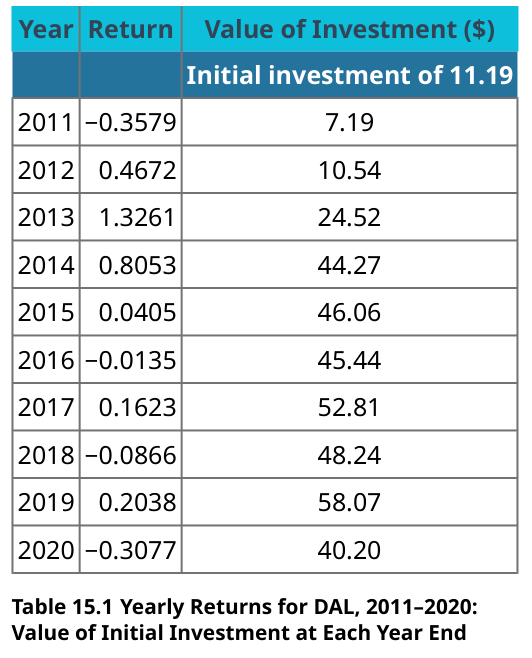
\includegraphics[width=0.7\linewidth]{gfx/m3l1_dahlquist_table15-1_dal_investment_value.png}
\par\smallskip{\small \textbf{Bảng 15.1:} Lợi suất hàng năm của DAL, 2011--2020: Giá trị khoản đầu tư ban đầu vào cuối mỗi năm}
\end{figure}

Mặc dù khoản đầu tư \$11.19 vào DAL đầu năm 2011 đã tăng lên \$40.20 vào cuối năm 2020, mức tăng trưởng này không nhất quán qua từng năm. Số tiền cổ phiếu đáng giá vào cuối mỗi năm cũng được trình bày trong Bảng 15.1. Trong năm 2011, lợi suất của DAL là $-35.79\%$, khiến giá trị khoản đầu tư giảm xuống $\$11.19 \times (1-0.3579) = \$7.19$. Năm tiếp theo, 2012, lợi suất của DAL là 46.72\%. Do đó, giá trị khoản đầu tư là $\$7.19 \times (1+0.4672) = \$10.54$ vào cuối năm 2012. Quá trình này tiếp diễn qua từng năm cổ phiếu được nắm giữ.

Lợi suất hàng năm kép suy ra từ công thức EAR và giá trị thời gian của tiền còn được gọi là lợi suất trung bình hình học (geometric average return). Lợi suất trung bình hình học được tính bằng công thức:

$$
R_{\text{GeomAvg}} = \left[ (1+R_1)(1+R_2)\cdots(1+R_N) \right]^{1/N} - 1
$$

trong đó $R_N$ là lợi suất của mỗi năm trong giai đoạn tính trung bình.

Phép tính lợi suất trung bình hình học cho DAL được trình bày ở cột bên phải của Bảng 15.2. (Chênh lệch nhỏ giữa lợi suất trung bình hình học 13.64\% với 13.65\% suy ra từ EAR và giá trị thời gian của tiền là do sai số làm tròn.)

\begin{figure}[H]
\centering
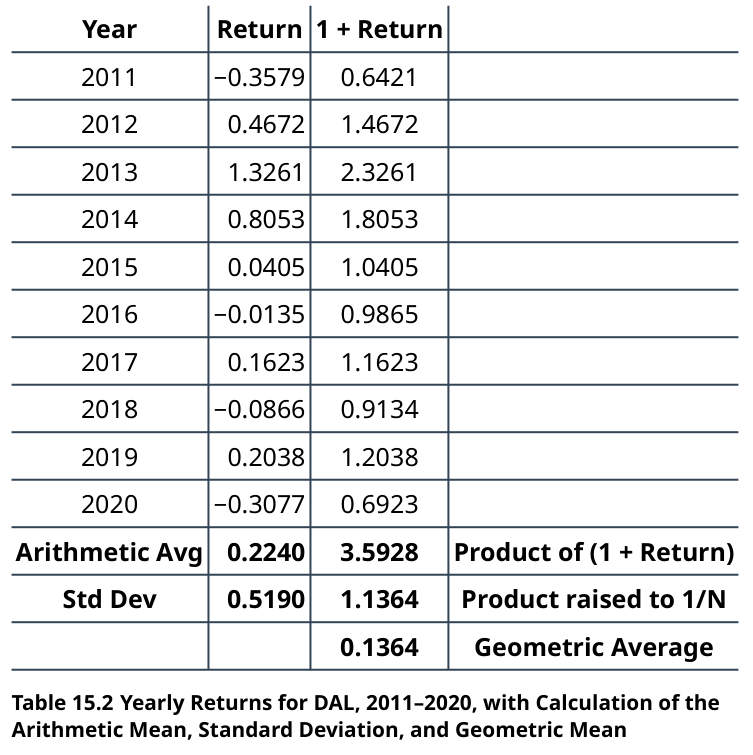
\includegraphics[width=0.75\linewidth]{gfx/m3l1_dahlquist_table15-2_dal_geometric_avg.png}
\par\smallskip{\small \textbf{Bảng 15.2:} Lợi suất hàng năm của DAL, 2011--2020, cùng phép tính Trung bình Số học, Độ lệch chuẩn và Trung bình Hình học}
\end{figure}

Nhìn vào Bảng 15.2, bạn sẽ nhận thấy lợi suất trung bình hình học khác với lợi suất trung bình (mean). Cộng từng lợi suất hàng năm và chia tổng cho 10 cho ra lợi suất trung bình hàng năm là 22.4\%. Con số 22.4\% này được gọi là lợi suất trung bình số học (arithmetic average return).

Lợi suất trung bình hình học sẽ nhỏ hơn lợi suất trung bình số học (trừ khi lợi suất của tất cả các năm giống hệt nhau). Điều này là do bản chất số học cơ bản của lãi kép. Hãy nghĩ về một ví dụ rất đơn giản trong đó bạn đầu tư \$100 trong hai năm. Nếu năm đầu tiên bạn có lợi suất dương 50\% và năm thứ hai lợi suất âm 50\%, bạn sẽ có lợi suất trung bình số học là $(50\%-50\%)/2 = 0\%$, nhưng bạn sẽ có lợi suất trung bình hình học là $[(1.5)(0.5)]^{1/2}-1 = -13.40\%$. Với lợi suất dương 50\% năm đầu tiên, bạn kết thúc năm với \$150. Năm thứ hai, bạn mất 50\% số dư đó và chỉ còn lại \$75.

Một sự thật quan trọng khác khi nghiên cứu lợi suất trung bình là thứ tự bạn kiếm được các lợi suất đó không quan trọng. Hãy xem xét điều gì sẽ xảy ra nếu lợi suất của hai năm bị đảo ngược, tức là bạn chịu lỗ 50\% trong năm đầu tư đầu tiên và lãi 50\% trong năm thứ hai. Với lợi suất $-50\%$ năm đầu tiên, bạn sẽ kết thúc năm đó chỉ với \$50. Sau đó, nếu \$50 đó sinh lợi 50\% dương ở năm thứ hai, bạn sẽ có số dư \$75 vào cuối giai đoạn hai năm. Lợi suất âm 50\% theo sau bởi lợi suất dương 50\% vẫn cho ra lợi suất trung bình số học 0\% và lợi suất trung bình hình học $-13.40\%$.

\begin{framed}
\textbf{THỰC HÀNH: Tính Lợi suất Trung bình Số học và Hình học}

Lợi suất hàng năm của CVS Health Corp. (CVS) cho giai đoạn 10 năm 2011--2020 được trình bày trong Bảng 15.3.

\begin{figure}[H]
\centering
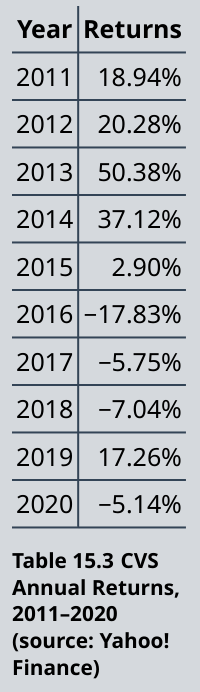
\includegraphics[width=0.4\linewidth]{gfx/m3l1_dahlquist_table15-3_cvs_annual_returns.png}
\par\smallskip{\small \textbf{Bảng 15.3:} Lợi suất hàng năm của CVS, 2011--2020 (nguồn: Yahoo! Finance)}
\end{figure}

Lợi suất trung bình số học trong thập kỷ đó là bao nhiêu? Lợi suất trung bình hình học trong thập kỷ đó là bao nhiêu?

\textbf{Lời giải:}

Xem Bảng 15.4 cho phép tính trung bình số học và trung bình hình học.

\begin{figure}[H]
\centering
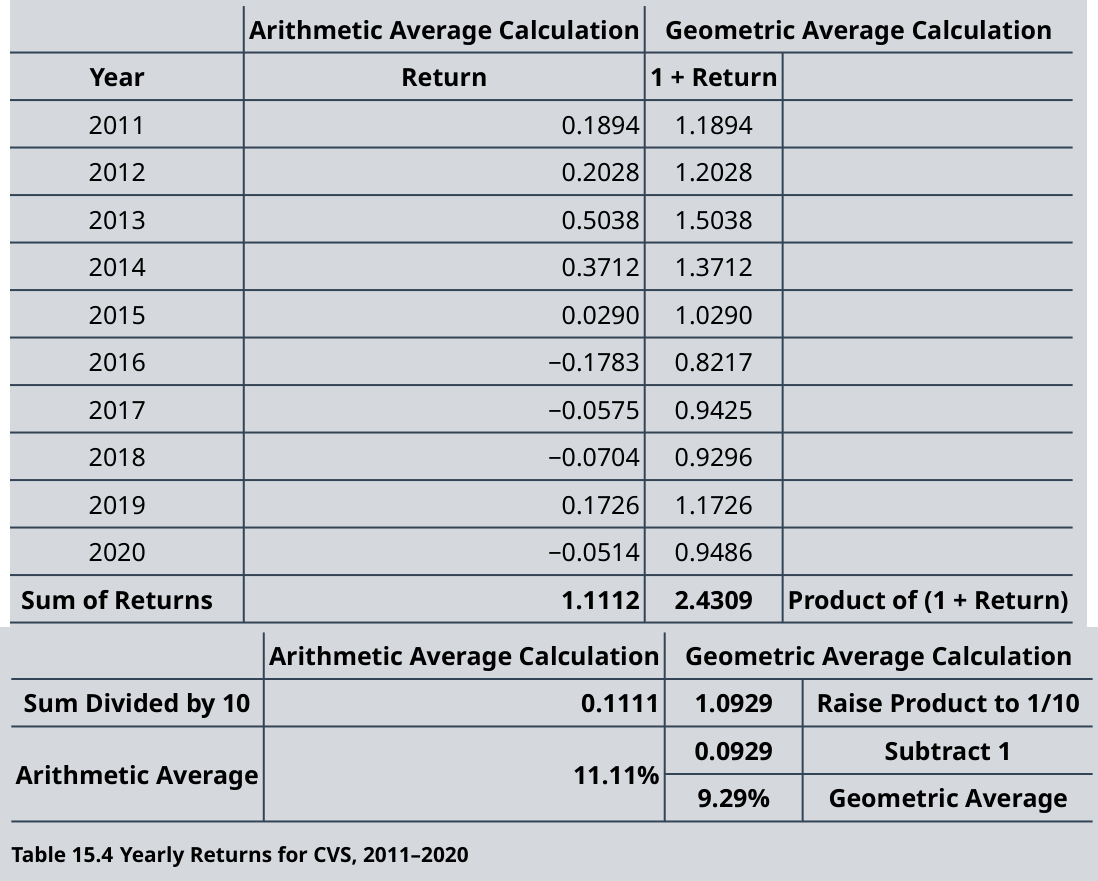
\includegraphics[width=0.85\linewidth]{gfx/m3l1_dahlquist_table15-4_cvs_avg_return_calc.png}
\par\smallskip{\small \textbf{Bảng 15.4:} Lợi suất hàng năm của CVS, 2011--2020}
\end{figure}

Lợi suất trung bình số học của CVS là 11.11\%, và lợi suất trung bình hình học là 9.29\%.
\end{framed}

Cả lợi suất trung bình số học và lợi suất trung bình hình học đều là các phép tính "đúng". Chúng chỉ trả lời các câu hỏi khác nhau. Trung bình hình học cho bạn biết thực tế bạn kiếm được bao nhiêu mỗi năm tính trung bình, theo lãi kép hàng năm. Nó hữu ích để tính mức tăng trưởng của một khoản đầu tư cụ thể qua thời gian. Trung bình số học cho bạn biết bạn kiếm được bao nhiêu trong một năm điển hình. Khi xem xét mô tả lịch sử của phân phối lợi suất và muốn dự đoán những gì nên kỳ vọng trong một năm cụ thể, trung bình số học là phép tính liên quan.

\subsection*{Đo lường Rủi ro}

Mặc dù lợi suất trung bình số học của Delta Airlines (DAL) giai đoạn 2011--2020 là 22.4\%, không có năm nào lợi suất đúng bằng 22.4\%. Thực tế, một số năm lợi suất cao hơn nhiều so với trung bình, chẳng hạn năm 2013, khi lợi suất là 132.61\%. Những năm khác, lợi suất âm, chẳng hạn năm 2011, khi lợi suất là $-35.79\%$. Nhìn vào lợi suất hàng năm trong Bảng 15.2, lợi suất của DAL biến động rất nhiều qua từng năm. Trong tài chính, độ biến động lợi suất này được coi là rủi ro.

\subsection*{Độ Biến động của Lợi suất}

Thước đo phổ biến nhất về độ biến động lợi suất trong tài chính là độ lệch chuẩn (standard deviation) của lợi suất. Độ lệch chuẩn của lợi suất DAL cho giai đoạn mẫu 2011--2020 là 51.9\%. Hãy nhớ rằng nếu phân phối chuẩn (đường cong hình chuông) mô tả lợi suất, thì 68\% (hay khoảng hai phần ba) thời gian, lợi suất trong một năm cụ thể sẽ nằm trong khoảng một độ lệch chuẩn phía trên và một độ lệch chuẩn phía dưới lợi suất trung bình số học. Với lợi suất trung bình 22.4\% của DAL, lợi suất thực tế hàng năm sẽ nằm đâu đó giữa $-29.5\%$ và $74.29\%$ trong hai trên ba năm. Một lợi suất rất cao trên 74.29\% sẽ xảy ra 16\% thời gian; một khoản lỗ rất lớn hơn 29.5\% cũng sẽ xảy ra 16\% thời gian.

Như bạn thấy, có một phạm vi rộng những gì có thể coi là một năm "điển hình" đối với DAL. Mặc dù ta có thể tính lợi suất trung bình, lợi suất trong bất kỳ năm cụ thể nào có khả năng khác với mức trung bình đó. Độ lệch chuẩn càng lớn, phạm vi lợi suất này càng lớn. Do đó, độ lệch chuẩn lớn hơn cho thấy độ biến động lợi suất lớn hơn và do đó rủi ro cao hơn.

\begin{framed}
\textbf{THỰC HÀNH: Tính Độ lệch chuẩn của Lợi suất}

Bạn đã tính lợi suất trung bình số học của CVS là 11.11\% cho giai đoạn 10 năm 2011--2020. Hãy tính độ lệch chuẩn của lợi suất CVS cho cùng giai đoạn (xem Bảng 15.5). Điều này cho bạn biết gì về những gì một nhà đầu tư vào CVS đã trải qua trong một năm điển hình của thập kỷ đó?

\textbf{Lời giải:}

\begin{figure}[H]
\centering
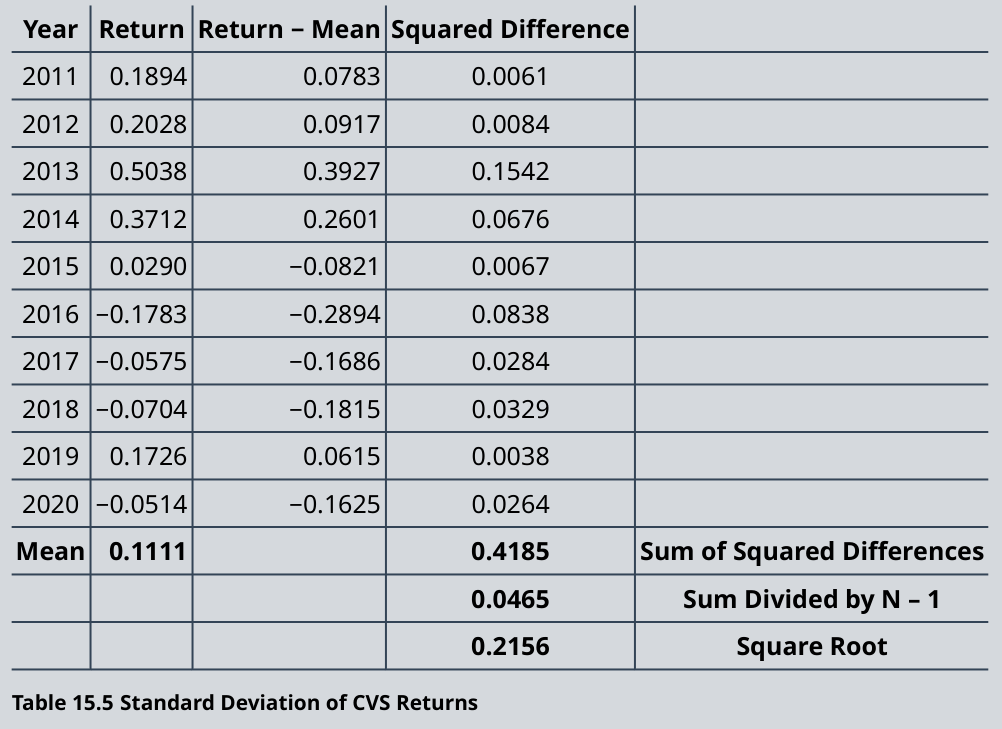
\includegraphics[width=0.55\linewidth]{gfx/m3l1_dahlquist_table15-5_cvs_stddev.png}
\par\smallskip{\small \textbf{Bảng 15.5:} Độ lệch chuẩn của Lợi suất CVS}
\end{figure}

Độ lệch chuẩn của lợi suất CVS trong giai đoạn mẫu 2011--2020 là 21.56\%. Với lợi suất trung bình số học 11.11\%, lợi suất sẽ nằm trong khoảng $-10.45\%$ và $32.67\%$ trong khoảng hai trên ba năm. Mặc dù lợi suất trung bình là 11.11\%, lợi suất trong một năm cụ thể có thể cao hơn hoặc thấp hơn nhiều so với mức trung bình đó. Thực tế, một khoản lỗ hơn 10.45\% được kỳ vọng xảy ra khoảng một lần mỗi sáu năm. Ngoài ra, khoảng một lần mỗi sáu năm, lợi suất lớn hơn 32.67\% cũng được kỳ vọng xảy ra.
\end{framed}

\subsection*{Rủi ro Đặc thù Doanh nghiệp}

Nhà đầu tư mua cổ phiếu với hy vọng cổ phiếu sẽ tăng giá trị và họ sẽ nhận lợi suất dương. Tuy nhiên, bạn có thể thấy rằng ngay cả với các công ty đã ổn định như ExxonMobil và CVS, lợi suất vẫn rất biến động. Nhà đầu tư không bao giờ có thể dự đoán hoàn hảo lợi suất của một cổ phiếu sẽ là bao nhiêu, hay thậm chí liệu nó có dương hay không.

Lợi suất hàng năm của bốn công ty — Delta Airlines (DAL), Southwest Airlines (LUV), ExxonMobil (XOM), và CVS Health Corp. (CVS) — được trình bày trong Bảng 15.6. Mỗi cổ phiếu này đều có những năm hiệu suất tốt hơn hoặc tệ hơn nhiều so với trung bình số học. Thực tế, không cổ phiếu nào có vẻ có một mức lợi suất "điển hình" lặp lại năm này qua năm khác.

\begin{figure}[H]
\centering
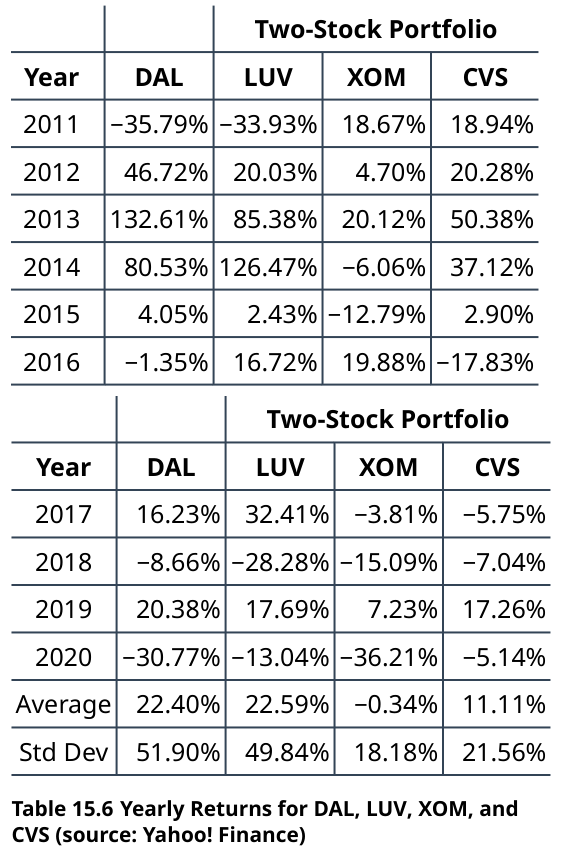
\includegraphics[width=0.75\linewidth]{gfx/m3l1_dahlquist_table15-6_yearly_returns.png}
\par\smallskip{\small \textbf{Bảng 15.6:} Lợi suất hàng năm của DAL, LUV, XOM và CVS (nguồn: Yahoo! Finance)}
\end{figure}

Hình 15.2 trình bày đồ thị lợi suất của từng cổ phiếu trong bốn cổ phiếu này theo năm. Trong đồ thị này, có thể dễ dàng thấy rằng DAL và LUV đều có độ biến động cao hơn, tức lợi suất biến thiên nhiều hơn qua từng năm, so với XOM hoặc CVS. Độ biến động cao hơn này khiến DAL và LUV có độ lệch chuẩn lợi suất cao hơn XOM hoặc CVS.

\begin{figure}[H]
\centering
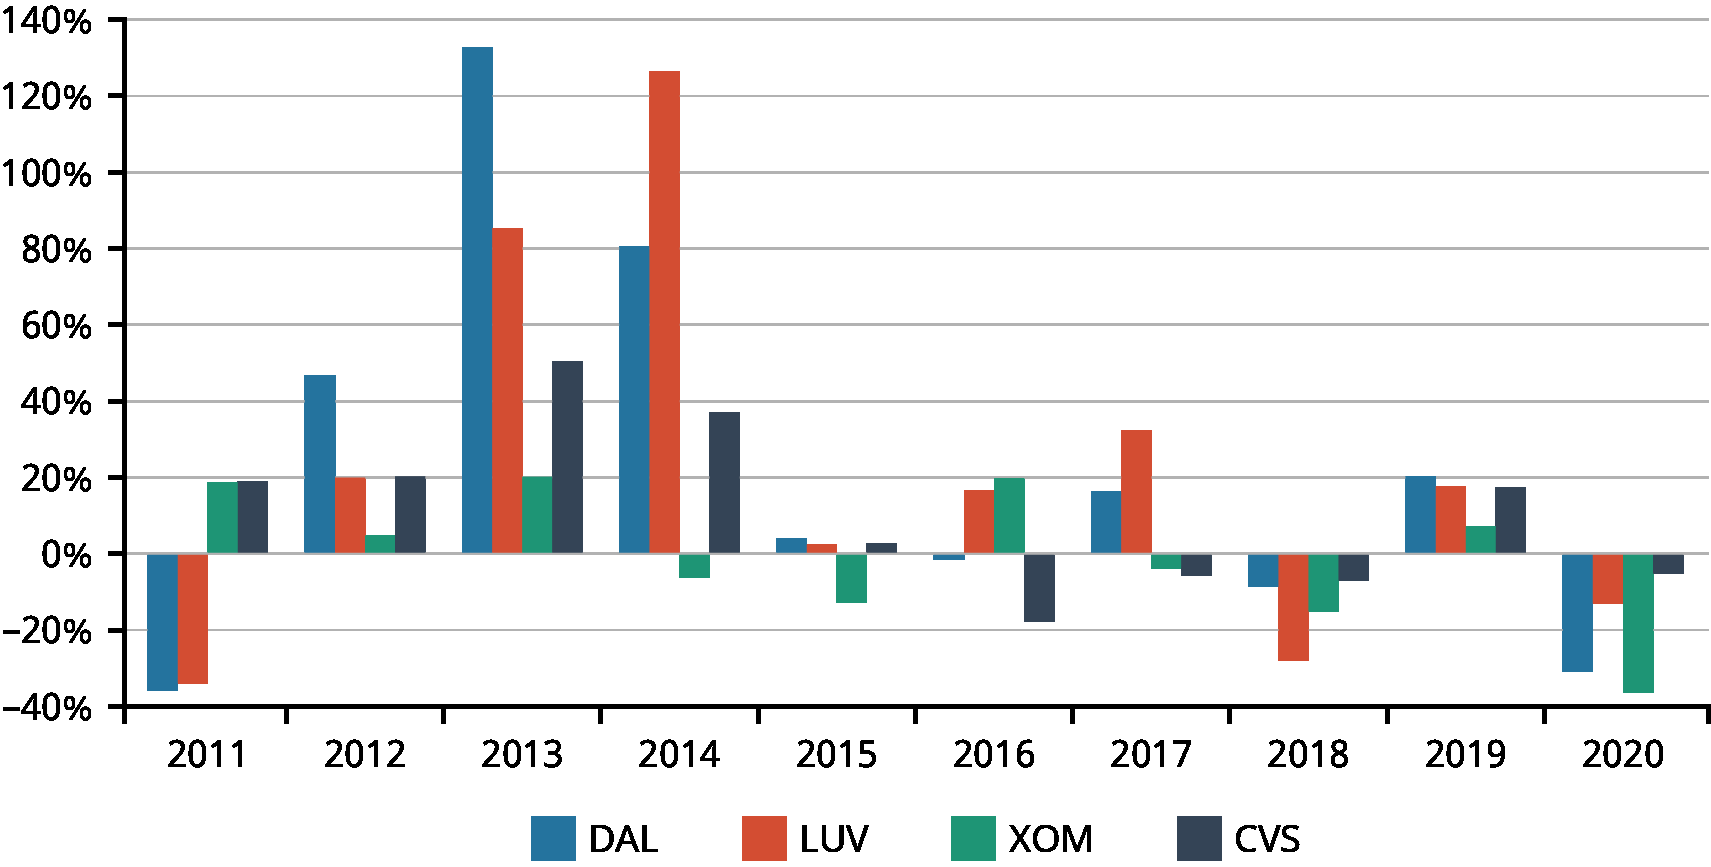
\includegraphics[width=\linewidth,height=0.6\textheight,keepaspectratio]{gfx/m3l1_dahlquist_fig15-2_yearly_returns.png}
\par\smallskip{\small \textbf{Hình 15.2:} Lợi suất hàng năm của DAL, LUV, XOM và CVS (nguồn dữ liệu: Yahoo! Finance)}
\end{figure}

Độ lệch chuẩn được coi là một thước đo rủi ro khi sở hữu một cổ phiếu. Độ lệch chuẩn lợi suất hàng năm của cổ phiếu càng lớn, lợi suất của cổ phiếu đó trong bất kỳ năm nào càng có khả năng lệch xa khỏi mức trung bình. Nói cách khác, lợi suất của cổ phiếu rất khó dự đoán. Mặc dù lợi suất của CVS biến thiên qua từng năm, nó không biến động mạnh như lợi suất của DAL hay LUV.

Tại sao lợi suất cổ phiếu lại biến động nhiều đến vậy? Giá trị cổ phiếu của một công ty thay đổi khi kỳ vọng về doanh thu và chi phí tương lai của công ty thay đổi. Những kỳ vọng này có thể thay đổi do nhiều sự kiện và thông tin mới. Tin tốt về một công ty thường dẫn đến giá cổ phiếu tăng. Ví dụ, DAL thông báo sẽ mở các tuyến bay mới và bay đến các thành phố trước đây chưa phục vụ cho thấy DAL sẽ có nhiều khách hàng hơn và doanh thu nhiều hơn trong tương lai. Hoặc nếu CVS thông báo đã đàm phán được giá thuê thấp hơn cho nhiều địa điểm của mình, nhà đầu tư sẽ kỳ vọng chi phí công ty giảm, dẫn đến lợi nhuận cao hơn. Những loại thông báo này thường đi kèm với giá cổ phiếu cao hơn. Ngược lại, nếu phi công và tiếp viên của DAL đàm phán được mức lương cao hơn, chi phí của DAL sẽ tăng, gây áp lực giảm lên lợi nhuận và giá cổ phiếu.

\begin{framed}
\textbf{LIÊN KẾT ĐẾN VIỆC HỌC: Peloton và Rủi ro}

Một ví dụ về cách tin tức có thể ảnh hưởng đến giá cổ phiếu xảy ra vào ngày 5/5/2021, khi Peloton thu hồi toàn bộ sản phẩm Tread+ và Tread sau cái chết thương tâm của một trẻ em và 70 ca chấn thương liên quan đến việc sử dụng sản phẩm. Ngày hôm trước, cổ phiếu Peloton giao dịch ở mức \$96.70/cổ phiếu. Giá cổ phiếu giảm khoảng 15\% khi việc thu hồi được công bố. Giá đóng cửa của cổ phiếu Peloton ngày 5/5 là \$82.62.
\end{framed}

\section{15.2 Rủi ro và Lợi suất của Nhiều Tài sản}

\subsection*{Mục tiêu học tập}
Sau khi hoàn thành mục này, bạn sẽ có thể:
\begin{itemize}
  \item Giải thích lợi ích của đa dạng hóa (diversification).
  \item Mô tả mối quan hệ giữa rủi ro và lợi suất đối với các danh mục đầu tư lớn.
  \item So sánh rủi ro đặc thù doanh nghiệp và rủi ro hệ thống.
  \item Thảo luận cách quy mô danh mục đầu tư ảnh hưởng đến rủi ro.
\end{itemize}

\subsection*{Đa dạng hóa}

Đến nay, chúng ta đã xem xét lợi suất và độ biến động của một cổ phiếu riêng lẻ. Tuy nhiên, hầu hết nhà đầu tư sở hữu cổ phiếu của nhiều công ty. Tập hợp cổ phiếu này được gọi là danh mục đầu tư (portfolio). Hãy cùng khám phá vì sao nhà đầu tư nên nắm giữ một danh mục cổ phiếu thay vì chỉ chọn một cổ phiếu yêu thích duy nhất để sở hữu.

Chúng ta đã thấy rằng nhà đầu tư sở hữu DAL có lợi suất trung bình hàng năm 20.87\% nhưng cũng có độ lệch chuẩn lớn 51.16\%. Nhà đầu tư dùng toàn bộ vốn để mua cổ phiếu DAL đã có kết quả cực kỳ tốt trong giai đoạn 2012--2014. Nhưng vào năm 2020, các nhà đầu tư đó đã mất gần một phần ba số tiền khi COVID-19 khiến việc đi lại bằng đường hàng không toàn cầu giảm mạnh. Để bảo vệ trước các kết quả cực đoan này, nhà đầu tư thực hành cái gọi là đa dạng hóa, tức nắm giữ nhiều loại cổ phiếu khác nhau trong danh mục đầu tư của mình.

Giả sử, ví dụ, bạn đã tiết kiệm được \$50,000 muốn đầu tư. Nếu bạn mua \$50,000 cổ phiếu DAL, bạn sẽ không được đa dạng hóa. Lợi suất của bạn sẽ chỉ phụ thuộc vào lợi suất của cổ phiếu DAL. Nếu thay vào đó, bạn dùng \$5,000 để mua cổ phiếu DAL và dùng \$45,000 còn lại để mua chín cổ phiếu khác, bạn đang đa dạng hóa. Lợi suất của bạn sẽ phụ thuộc không chỉ vào lợi suất của DAL mà còn vào lợi suất của chín cổ phiếu khác trong danh mục. Nhà đầu tư thực hành đa dạng hóa để quản lý rủi ro.

Điều này tương tự câu nói "Đừng bỏ hết trứng vào một giỏ." Nếu bạn để tất cả trứng vào một giỏ và giỏ đó vỡ, tất cả trứng của bạn sẽ rơi và vỡ. Nếu bạn phân tán trứng ra nhiều giỏ, khó có khả năng tất cả các giỏ đều vỡ và tất cả trứng đều bể. Một giỏ có thể vỡ, và bạn sẽ mất số trứng trong giỏ đó, nhưng bạn vẫn còn những giỏ trứng khác. Ý tưởng tương tự cũng đúng với đầu tư. Nếu bạn sở hữu cổ phiếu của một công ty làm ăn kém, thậm chí phá sản, bạn sẽ mất số tiền đã đặt vào khoản đầu tư cụ thể đó. Tuy nhiên, với một danh mục đa dạng hóa, bạn không mất toàn bộ số tiền vì tiền của bạn được phân tán qua nhiều công ty khác nhau.

\begin{framed}
\textbf{LIÊN KẾT ĐẾN VIỆC HỌC: Đa dạng hóa}

Fidelity Investments Inc. là một công ty dịch vụ tài chính đa quốc gia và là một trong những công ty quản lý tài sản lớn nhất thế giới. Trong video giáo dục dành cho nhà đầu tư này, Fidelity giải thích đa dạng hóa là gì và nó ảnh hưởng thế nào đến danh mục đầu tư của nhà đầu tư.
\end{framed}

Bảng 15.7 trình bày lợi suất của nhà đầu tư đặt 50\% tiền vào DAL và 50\% còn lại vào LUV, XOM, hoặc CVS. Lưu ý rằng độ lệch chuẩn lợi suất thấp hơn đối với các danh mục hai cổ phiếu so với DAL là một khoản đầu tư riêng lẻ.

\begin{figure}[H]
\centering
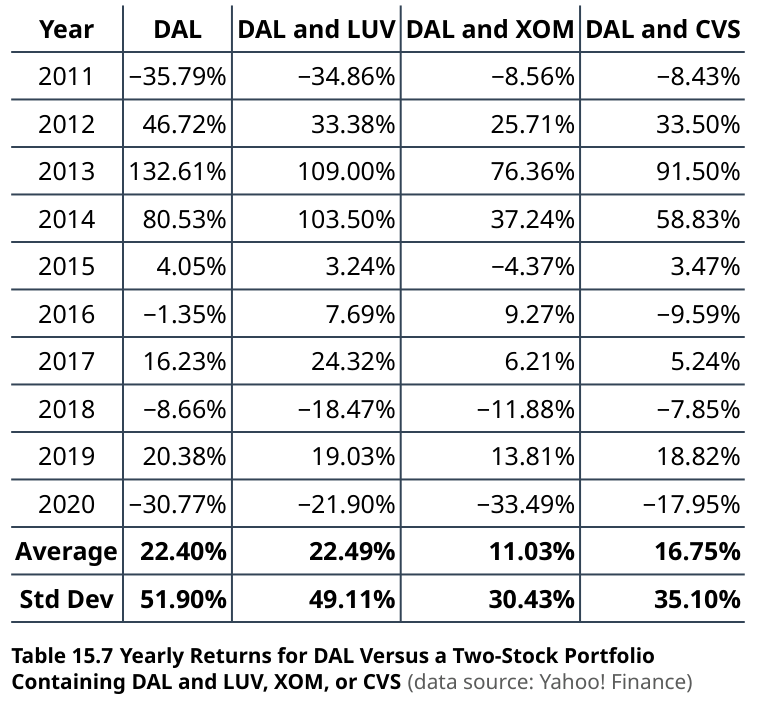
\includegraphics[width=0.85\linewidth]{gfx/m3l1_dahlquist_table15-7_two_stock_portfolio_returns.png}
\par\smallskip{\small \textbf{Bảng 15.7:} Lợi suất hàng năm của DAL so với Danh mục Hai Cổ phiếu gồm DAL và LUV, XOM, hoặc CVS (nguồn dữ liệu: Yahoo! Finance)}
\end{figure}

Khi nhà đầu tư đa dạng hóa danh mục của mình, độ biến động của một cổ phiếu cụ thể trở nên kém quan trọng hơn. XOM có những năm tốt với lợi suất trên trung bình và những năm xấu với lợi suất dưới trung bình (thậm chí âm), giống như DAL. Nhưng những năm mà các lợi suất trên/dưới trung bình đó xảy ra không phải lúc nào cũng giống nhau giữa hai công ty. Ví dụ, năm 2014, lợi suất của DAL lớn hơn 80\%, trong khi lợi suất của XOM âm. Mặt khác, năm 2011, khi DAL có lợi suất $-35.15\%$, XOM lại có lợi suất dương. Khi nắm giữ nhiều hơn một cổ phiếu, lãi ở một cổ phiếu có thể bù đắp lỗ ở cổ phiếu khác, làm giảm bớt một phần độ biến động.

Khi nhà đầu tư chỉ nắm giữ một cổ phiếu, độ biến động của cổ phiếu đó đóng góp 100\% vào độ biến động của danh mục. Khi nắm giữ hai cổ phiếu, độ biến động của mỗi cổ phiếu đóng góp vào độ biến động của danh mục. Tuy nhiên, độ biến động của danh mục không đơn giản là trung bình độ biến động của từng cổ phiếu nắm giữ độc lập. Mức độ tương quan giữa hai cổ phiếu, hay chúng di chuyển cùng nhau đến đâu, sẽ ảnh hưởng đến độ biến động của danh mục.

Bạn sẽ nhớ lại từ nghiên cứu về tương quan trong Phân tích Hồi quy trong Tài chính rằng hệ số tương quan mô tả cách hai biến di chuyển tương đối với nhau. Hệ số tương quan bằng 1 nghĩa là có tương quan dương hoàn hảo giữa hai biến, trong khi hệ số tương quan bằng $-1$ nghĩa là hai biến di chuyển hoàn toàn ngược nhau. Các cổ phiếu cùng ngành thường có xu hướng tương quan mạnh hơn các cổ phiếu ở các ngành rất khác nhau. Trong giai đoạn 2011--2020, hệ số tương quan giữa DAL và LUV là 0.87, hệ số tương quan giữa DAL và XOM là 0.35, và hệ số tương quan giữa DAL và CVS là 0.79. Kết hợp các cổ phiếu không tương quan dương hoàn hảo trong một danh mục sẽ giảm rủi ro.

Lưu ý rằng nhà đầu tư sở hữu DAL và LUV từ 2011 đến 2020 sẽ có độ lệch chuẩn danh mục thấp hơn, nhưng không thấp hơn nhiều, so với nhà đầu tư chỉ sở hữu DAL. Vì hệ số tương quan nhỏ hơn 1, độ lệch chuẩn giảm xuống. Tuy nhiên, vì hai cổ phiếu cùng ngành và chịu ảnh hưởng bởi nhiều vấn đề kinh tế giống nhau, hệ số tương quan tương đối cao, và việc kết hợp hai cổ phiếu này chỉ giảm rủi ro một phần nhỏ.

Điều này là vì, là các hãng hàng không, DAL và LUV đối mặt với nhiều điều kiện thị trường giống nhau. Trong những năm kinh tế mạnh, thời tiết tốt, giá nhiên liệu thấp, và người dân đi lại nhiều, cả hai công ty đều làm ăn tốt. Khi điều gì đó như thời tiết xấu làm giảm lượng di chuyển hàng không trong nhiều tuần, cả hai công ty đều bị ảnh hưởng. Bằng cách nắm giữ LUV bên cạnh DAL, nhà đầu tư có thể giảm phơi nhiễm với rủi ro đặc thù của DAL (có thể là vấn đề với hệ thống đặt vé của DAL), nhưng họ không giảm được phơi nhiễm với rủi ro liên quan đến ngành hàng không (có thể là giá nhiên liệu máy bay tăng). DAL và LUV có xu hướng có lợi suất dương trong cùng những năm và lợi suất âm trong cùng những năm.

Mặt khác, nhà đầu tư thêm XOM vào danh mục của họ thấy độ lệch chuẩn thấp hơn đáng kể so với những người chỉ nắm giữ DAL. Trong những năm giá nhiên liệu máy bay tăng, gây hại cho lợi nhuận của cả DAL và LUV, XOM có khả năng có lợi nhuận cao. Đa dạng hóa danh mục qua các công ty ít tương quan hơn sẽ giảm độ lệch chuẩn của danh mục nhiều hơn.

\begin{framed}
\textbf{LIÊN KẾT ĐẾN VIỆC HỌC: Cách Xây dựng một Danh mục Đa dạng hóa}

Nhân vật truyền hình, cựu quản lý quỹ phòng hộ, và tác giả Jim Cramer khuyến khích nhà đầu tư xây dựng một danh mục đa dạng hóa, không quá 20\% danh mục trong một ngành. Ông đề xuất nhà đầu tư có thể xây dựng danh mục đa dạng hóa bằng cách mua từ năm đến mười cổ phiếu.
\end{framed}

\subsection*{Quy mô Danh mục và Rủi ro}

Khi bạn thêm nhiều cổ phiếu vào danh mục, độ biến động, hay độ lệch chuẩn, của danh mục giảm xuống. Độ biến động của từng tài sản riêng lẻ trở nên ngày càng kém quan trọng. Như đã thảo luận trước đó, rủi ro liên quan đến các sự kiện của một công ty cụ thể được gọi là rủi ro đặc thù doanh nghiệp, hay rủi ro phi hệ thống (unsystematic risk). Ví dụ về rủi ro phi hệ thống bao gồm một công ty đối mặt với vụ kiện trách nhiệm sản phẩm, một công ty phát minh sản phẩm mới, hoặc phát hiện gian lận kế toán. Nắm giữ một danh mục cổ phiếu nghĩa là nếu một công ty bạn đầu tư phá sản do quản lý kém, bạn không mất toàn bộ tiền tiết kiệm vì một phần tiền của bạn được đầu tư vào các công ty khác. Đa dạng hóa danh mục bảo vệ bạn khỏi bị ảnh hưởng đáng kể bởi rủi ro phi hệ thống.

Tuy nhiên, có một mức mà rủi ro danh mục không giảm xuống dưới đó, dù danh mục có đa dạng hóa đến đâu. Rủi ro không bao giờ biến mất này được gọi là rủi ro hệ thống (systematic risk). Rủi ro hệ thống là rủi ro của việc nắm giữ danh mục thị trường.

Chúng ta đã nói về lý do lợi suất của một công ty có thể biến động; ví dụ, việc công ty phát hiện một công nghệ mới hoặc bị kiện trách nhiệm sản phẩm sẽ ảnh hưởng đặc thù đến công ty đó. Cũng có những sự kiện ảnh hưởng rộng rãi đến toàn thị trường chứng khoán. Thay đổi trong chính sách tiền tệ và lãi suất của Cục Dự trữ Liên bang ảnh hưởng đến tất cả các công ty. Các sự kiện địa chính trị, bão lớn, và đại dịch cũng có thể ảnh hưởng đến toàn bộ thị trường. Nhà đầu tư cổ phiếu không thể tránh khỏi loại rủi ro này. Rủi ro không thể tránh khỏi này chính là rủi ro hệ thống mà nhà đầu tư cổ phiếu phải gánh chịu. Rủi ro hệ thống này không thể loại bỏ thông qua đa dạng hóa.

Ngoài ra, theo nghiên cứu của Meir Statman, độ lệch chuẩn của một danh mục giảm nhanh khi số lượng cổ phiếu trong danh mục tăng từ một lên hai hoặc ba. Tăng quy mô danh mục giúp giảm độ lệch chuẩn, và do đó giảm rủi ro, của danh mục. Tuy nhiên, khi danh mục tăng quy mô, mức rủi ro giảm được khi thêm một cổ phiếu nữa vào danh mục sẽ giảm dần. Một nhà đầu tư cần bao nhiêu cổ phiếu để danh mục được đa dạng hóa tốt? Không có con số chính xác mà tất cả các nhà quản lý tài chính đều đồng ý. Một danh mục gồm 15 cổ phiếu tương quan cao sẽ mang lại ít lợi ích đa dạng hóa hơn một danh mục gồm 10 cổ phiếu có hệ số tương quan thấp hơn. Một danh mục gồm American Airlines, Spirit Airlines, United Airlines, Southwest Airlines, Delta Airlines, và Jet Blue, cùng một vài cổ phiếu khác, không được đa dạng hóa tốt vì tập trung nặng vào ngành hàng không. Thuật ngữ danh mục đa dạng hóa là một khái niệm tương đối, nhưng nhà đầu tư bình thường có thể tạo một danh mục đa dạng hóa hợp lý với khoảng một tá cổ phiếu.
